% !TeX encoding = UTF-8
% !TeX program = xelatex
% !TeX spellcheck = en_US

\documentclass[degree=master]{thuthesis}
  % 学位 degree:
  %   doctor | master | bachelor | postdoc
  % 学位类型 degree-type:
  %   academic（默认）| professional
  % 语言 language
  %   chinese（默认）| english

% 论文基本配置，加载宏包等全局配置
\usepackage{pdfpages} % 导入宏包
% !TeX root = ./thuthesis-example.tex

% 论文基本信息配置（长沙理工大学硕士学位论文）

\thusetup{
  %******************************
  % 注意：
  %   1. 配置里面不要出现空行
  %   2. 不需要的配置信息可以删除
  %   3. 建议先阅读文档中所有关于选项的说明
  %******************************
  %
  % 输出格式
  output = electronic,
  %
  % 标题
  title  = {自动驾驶汽车自监督点云预测算法改善及应用研究},
  title* = {Research on the Improvement and Application of Self-Supervised Point Cloud Prediction Algorithms for Autonomous Vehicles},
  %
  % 学位类别
  degree-category  = {机械硕士},
  degree-category* = {Master of Engineering},
  %
  % 培养单位
  department = {汽车与机械工程学院},
  %
  % 学科
  discipline  = {机械工程},
  discipline* = {Mechanical Engineering},
  %
  % 姓名
  author  = {冯荣英},
  author* = {Feng Rongying},
  %
  % 指导教师
  supervisor  = {杜荣华, 教授},
  supervisor* = {Professor Du Ronghua},
  %
  % 副指导教师
  associate-supervisor  = {高凯, 副教授},
  associate-supervisor* = {Associate Professor Gao Kai},
  %
  % 日期
  date = {2024-04},
  %
  % 不生成书脊
  include-spine = false,
}

% 载入所需的宏包

% 定理类环境宏包
\usepackage{amsthm}

\thusetup{
  math-font  = xits,
}

% 表格加脚注
\usepackage{threeparttable}

% 表格中支持跨行
\usepackage{multirow}

% 跨页表格
\usepackage{longtable}

% 算法
\usepackage{algorithm}
\usepackage{algorithmic}

% 量和单位
\usepackage{siunitx}

% 参考文献使用 BibTeX + natbib 宏包（顺序编码制）
\usepackage[sort]{natbib}
\bibliographystyle{thuthesis-numeric}

% 定义所有的图片文件在 figures 子目录下
\graphicspath{{figures/}}

% 数学命令
\makeatletter
\newcommand\dif{%
  \mathop{}\!%
  \ifthu@math@style@TeX
    d%
  \else
    \mathrm{d}%
  \fi
}
\makeatother

% 载入长沙理工大学格式覆盖
\usepackage{csust-format}

% hyperref 宏包在最后调用
\usepackage{hyperref}



\begin{document}

% 封面（如不需要THUThesis封面，可注释掉）
% \maketitle

% 使用授权的说明（如不需要可注释掉）
% \copyrightpage

% ==================== 前置部分 ====================
\frontmatter


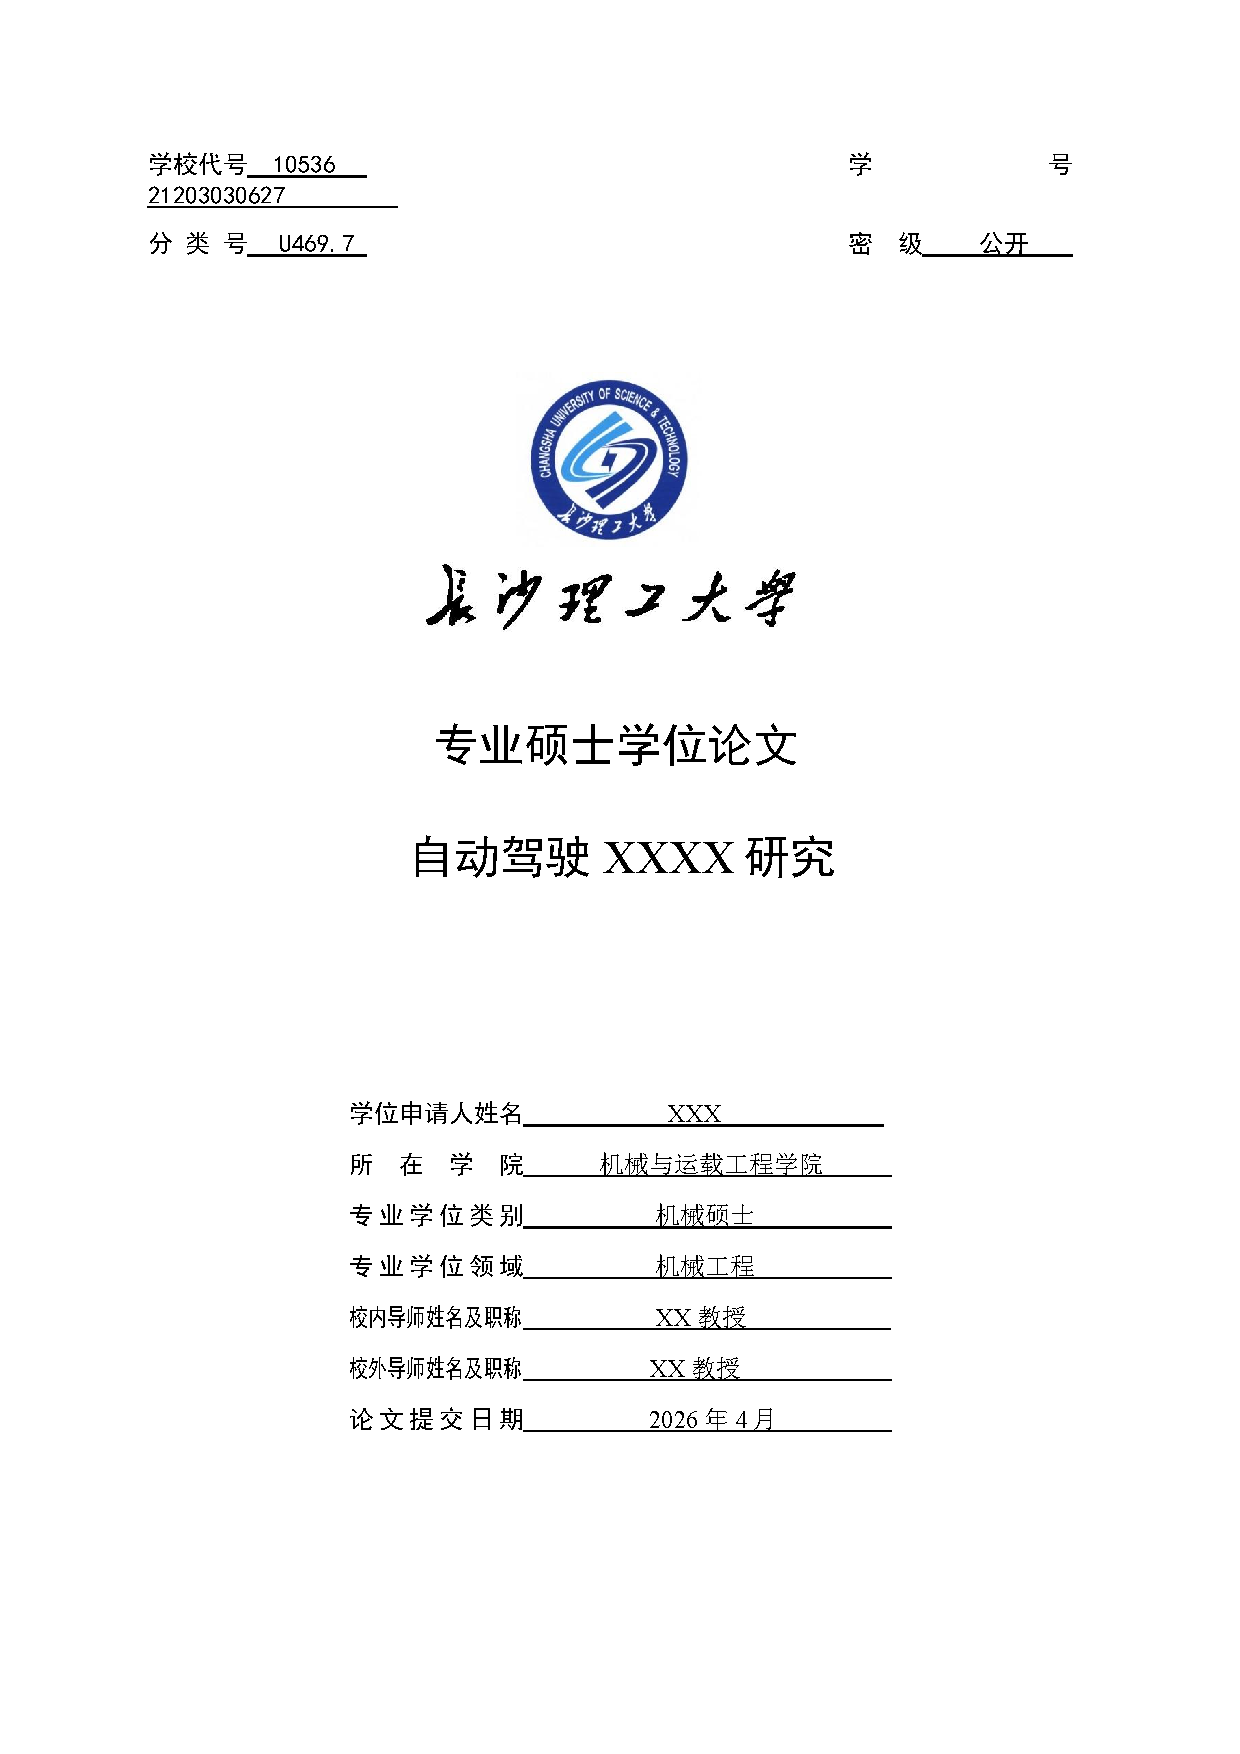
\includepdf[pages=-]{data/fengmian.pdf}


% 中英文摘要



% !TeX root = ../thuthesis-example.tex

% 中英文摘要和关键字

\begin{abstract}
  随着学习、工作节奏的不断加快，用户对时间管理、日常记录和个人财务管理的需求日益增长，但现有软件大多功能单一、平台割裂，难以同时满足专注计时、过程留痕和消费统计等综合需求。针对上述问题，本文结合当前已完成的项目，设计并实现了一套基于Qt框架的番茄计时与记账日记系统。系统采用C++作为开发语言，以Qt Widgets构建桌面图形界面，整体由登录会话、番茄计时、正向计时、日记记录、记账录入、数据统计、主题切换及扩展工具等模块组成。在数据管理方面，系统采用本地文件持久化策略：日记与专注记录以文本形式进行存储，记账数据采用JSON对象逐行写入的方式保存，从而兼顾实现成本、可读性与维护便利性。在功能实现方面，系统利用QTimer完成番茄计时与正向计时逻辑，利用QTableWidget完成账单展示与编辑，利用QMenu和QPropertyAnimation实现右键菜单及动画交互，利用自定义绘制的饼状图和柱状图对消费类型、周月专注时长及账单统计结果进行可视化表达。测试结果表明，该系统界面响应及时、功能运行稳定、数据读写正确，能够较好地满足个人用户在专注管理、日常记录与基础财务分析方面的实际需要。本文的研究与实现对于轻量级个人信息管理软件的开发具有一定的工程参考价值。

  % 关键词用"英文逗号"分隔，输出时会自动处理为正确的分隔符
  \thusetup{
    keywords = {Qt, C++, 番茄工作法, 记账系统, 数据可视化},
  }
\end{abstract}

\begin{abstract*}
  With the acceleration of study and work rhythm, users increasingly need an integrated desktop application that can support focus management, diary recording, and personal accounting at the same time. However, most existing tools are functionally fragmented and usually focus on only one specific scenario. To address this problem, this paper designs and implements a Pomodoro timing, accounting, and diary system based on the Qt framework. The system is developed in C++ and built with Qt Widgets. It consists of multiple modules, including user session management, Pomodoro timer, stopwatch, diary recording, accounting input, statistical analysis, theme switching, and several auxiliary tools. In terms of data persistence, the system adopts a lightweight local storage strategy. Diary and focus records are stored in text files, while accounting records are serialized as JSON objects and saved line by line, which improves portability and simplifies maintenance. In terms of interaction design, QTimer is used to control timing tasks, QTableWidget is used to display and manage accounting records, QMenu together with QPropertyAnimation is used to support context menu interaction, and custom pie charts and bar charts are used to visualize focus duration and consumption distribution. Functional testing shows that the system is stable, responsive, and practical. It can effectively assist users in improving concentration efficiency, recording daily life, and managing personal expenses. The project provides a useful reference for the design and implementation of lightweight personal information management software.

  \thusetup{
    keywords* = {Qt, C++, Pomodoro Technique, Accounting System, Data Visualization},
  }
\end{abstract*}


% 目录
\tableofcontents

% 插图和附表清单（根据需要取消注释）
% \listoffigures
% \listoftables

% 符号对照表（根据需要取消注释）
% \input{data/denotation}


% ==================== 正文部分 ====================
\mainmatter
% !TeX root = ../thuthesis-example.tex
\chapter{绪论}

\section{研究背景与意义}

\subsection{研究背景}
在数字化学习和办公环境中，时间管理、日程留痕和个人消费管理已经成为大学生和普通办公用户最常见的三类需求。当前市场上的相关应用虽然数量较多，但多数产品仅覆盖其中一种功能，例如番茄钟软件只提供倒计时服务，记账软件只关注收支录入，日记软件则更偏向文本记录，用户往往需要在多个应用之间频繁切换，导致信息分散、使用成本升高，也不利于形成连续、统一的个人行为数据。基于此，设计一套能够同时支持番茄计时、日记记录和基础记账分析的桌面应用系统具有较强的现实意义。

\subsection{研究意义}
本课题的研究意义主要体现在两个方面。其一，从应用价值角度看，该系统能够帮助用户在同一平台内完成专注计时、日记留存和消费管理，提高信息整合程度，增强使用连贯性。其二，从工程实践角度看，本课题以C++和Qt为核心技术路线，围绕界面设计、数据组织、模块协作、图表可视化和交互优化等内容展开实现，具有较强的软件工程训练价值。通过该项目，可以系统地验证桌面端轻量级个人信息管理软件的可行实现路径，为同类应用的开发提供参考。
从毕业设计的角度进一步分析，本系统兼具“功能完整性”和“技术可展示性”两方面特点。一方面，系统覆盖了用户登录、信息记录、数据统计、界面优化等多个完整业务流程，能够体现需求分析、系统设计、编码实现和测试验证的完整开发过程；另一方面，系统涉及Qt事件机制、定时器、文件系统、JSON序列化、自定义绘图、主题切换等多项关键技术，具备较强的综合训练意义。因此，本课题不仅适合用于实际场景中的个人效率管理，也能够较好地体现计算机科学与技术专业学生在桌面软件开发方向上的综合能力。

\section{国内外研究现状}

\subsection{国外研究现状}
国外在时间管理和个人效率工具方面起步较早，番茄工作法相关应用和任务管理工具已经较为成熟，一些产品还结合了统计图表、提醒机制和云同步能力，强调跨终端协同与用户行为数据分析。同时，国外桌面应用开发在跨平台框架和模块化设计方面积累了大量经验，Qt等技术方案被广泛应用于高性能桌面软件开发。

\subsection{国内研究现状}
国内相关软件产品在移动端发展迅速，围绕轻量记账、习惯打卡和时间管理形成了较为丰富的应用生态，但桌面端产品整体较少，且很多系统偏重商业化运营，存在功能堆叠、广告较多、数据导出受限等问题。对高校毕业设计而言，基于本地化存储与自主可控架构实现一套可独立运行的桌面系统，更具有研究与实践价值。

\subsection{现有问题分析}
综合现有产品可以发现，当前系统主要存在以下问题：一是功能分散，时间管理、日记与记账相互独立；二是部分系统对云端依赖程度较高，不利于隐私保护；三是桌面端产品在交互细节、图表展示和主题适配方面仍有提升空间。因此，本文选择以“集成化、轻量化、本地化”为目标，设计并实现番茄计时与记账日记系统。
此外，现有很多产品在“数据关联性”方面做得不够充分。例如，用户完成一次专注任务后，往往无法方便地将该事件与当天的日记内容和消费行为放在同一视角下观察，这使得个人行为数据之间缺乏关联。对于本项目而言，将专注记录、日记文本与账单信息纳入同一套本地管理体系，不仅可以提高软件实用性，也为后续进行更复杂的行为统计分析奠定了基础。

\sectionsection{研究内容与论文结构}

\subsection{研究内容}
本文围绕一个基于Qt的桌面系统展开研究与实现，主要内容包括：设计用户登录与会话机制；实现番茄计时和正向计时功能；构建日记记录和本地文件存储流程；新增记账模块并完成账单的录入、展示、编辑与删除；设计数据统计页面，通过饼状图和柱状图展示专注数据与消费分布；完成夜间主题、右键菜单和动画等交互优化；最后通过测试验证系统的可用性与稳定性。
在研究方法上，本文采用“需求驱动、逐步实现、测试验证”的开发路径。首先从用户日常使用场景出发，对系统所需功能进行抽象与拆分；其次根据Qt框架特点进行界面与逻辑分层实现；最后通过人工测试与QTest自动化测试相结合的方式，对关键功能进行验证。这样的研究过程既符合软件工程的开发规律，也便于将项目实现过程转化为较为完整的论文表达。

\subsection{论文结构安排}
本文共分为五章。第一章介绍研究背景、意义及国内外现状；第二章对系统需求和关键技术方案进行分析与比较；第三章重点阐述系统总体架构及各功能模块的设计与实现；第四章对系统进行测试并分析结果；第五章对全文进行总结，并给出后续改进方向。
% !TeX root = ../thuthesis-example.tex
\chapter{系统需求分析与方案论证}

\section{系统需求分析}

\subsection{功能需求分析}
结合项目当前实现，系统主要包含以下功能需求：
\begin{enumerate}
    \item 用户登录后能够进入统一主界面，并在多个功能页之间切换；
    \item 番茄计时模块支持任务名称输入、专注时长设置、休息时长设置、开始、暂停、继续和提前结束；
    \item 正向计时模块能够记录普通专注事件，并将统计结果写入本地数据文件；
    \item 日记模块能够按日期保存与读取文本内容，支持用户长期积累个人记录；
    \item 记账模块支持消费事项、金额和类型的录入，支持账单列表查看、编辑和删除；
    \item 统计模块能够对周、月等时间范围内的专注数据和消费数据进行汇总，展示图表和关键统计量；
    \item 系统应支持日间主题和夜间主题切换，以改善不同环境下的视觉体验。
\end{enumerate}
为了使系统具备更好的使用连续性，各模块之间还需要满足基本的数据联动要求。例如，番茄计时和正向计时产生的专注事件应自动进入本地记录文件，供日记模块展示和统计模块计算；记账模块录入的数据应当能够被统计模块实时读取并重新绘制图表；主题切换操作应对各页面和控件保持统一生效，避免界面风格割裂。由此可见，本系统的功能需求并非简单的模块堆叠，而是强调功能之间的协同工作能力。

\subsection{非功能需求分析}
在非功能层面，系统需要满足以下要求：首先，界面交互应清晰直观，便于普通用户快速上手；其次，系统运行应保持较好的响应性，避免在计时刷新、文件读写和图表绘制过程中出现明显卡顿；再次，数据存储应以本地化为主，降低部署与使用门槛；最后，系统结构应具备较好的模块化特征，便于后续扩展同步功能、数据库功能和更多工具模块。
除此之外，系统还需要满足一定的可维护性和可扩展性要求。由于毕业设计项目往往会在后续继续迭代，因此代码结构应尽量清晰，页面类、服务类和数据结构之间的职责划分应当明确。以当前项目为例，用户会话由独立的Session对象维护，数据读写由DataStore、DiaryStore和AccountingStore等服务类封装，统计逻辑则由StatsService和AccountingStatsService单独负责，这种分工方式有利于减少业务耦合度，并为后续引入数据库、云同步或更复杂的分析模型提供基础。

\section{关键技术与方案比较}

\subsection{GUI框架选型}
在桌面图形界面技术的选择上，本文对Qt、Electron和WPF进行了比较。Electron开发效率较高，但资源占用相对较大；WPF在Windows平台具有较好的开发体验，但跨平台能力有限；Qt则兼顾了性能、跨平台能力和组件丰富度，特别适合毕业设计类桌面系统开发。因此，本文最终选择Qt Widgets作为界面开发框架。
具体而言，Qt Widgets 提供了QMainWindow、QTabWidget、QTableWidget、QMenu、QToolBar、QCalendarWidget等大量成熟控件，能够快速搭建功能型桌面应用界面。更重要的是，Qt拥有稳定的信号与槽机制，便于描述页面内外的交互关系。例如，登录页面可通过发出登录成功信号进入主窗口，记账页面可通过动作信号响应编辑和删除操作，统计页面可通过按钮与图表点击事件完成图形切换与详情展示。这些特性使Qt在本项目中具备较高的开发效率与实现灵活性。

\subsection{数据存储方案比较}
在数据存储方案方面，可选方案主要包括关系数据库、本地文本文件和JSON文件。考虑到本系统定位为轻量级个人桌面工具，数据规模有限、部署环境简单，若直接引入数据库会增加配置与维护成本。因此，系统最终采用混合本地文件存储策略：专注记录与日记内容使用文本文件保存，便于按日期管理；记账数据则采用JSON对象逐行存储，既保留结构化特征，又降低解析复杂度。
该方案还有一个显著优点，即可视化和调试过程更加直接。开发者可以直接打开对应用户目录下的文件查看原始数据，有利于快速定位问题和验证功能效果。对于毕业设计项目而言，这种方式比完整引入数据库系统更适合当前规模，也更符合“轻量、直观、可演示”的实现目标。当然，这种方案的局限性也较为明显，例如复杂查询能力有限、缺少事务和并发控制，因此在后续展望部分，本文也提出了引入SQLite等数据库的改进方向。

\subsection{图表实现方案比较}
图表功能可通过引入第三方图表库实现，也可基于Qt绘图机制自行开发。第三方库开发速度较快，但会增加项目依赖；自定义绘制虽然实现复杂度较高，但更容易控制样式、交互和主题适配。结合本项目规模和教学实践要求，系统最终采用自定义饼状图和柱状图组件实现数据可视化，以增强对绘制流程和事件交互的掌握。
从系统效果来看，自定义图表组件不仅能够绘制静态图形，还能够与页面交互逻辑结合。例如，统计页面可以根据时间范围切换不同数据源，并将汇总结果同步展示到饼状图和柱状图中；用户点击图形元素后，还可以触发对应的数据详情展示。这种“绘制+交互”的设计方式，更有利于体现项目的工程实现能力，也使系统在展示环节更具完整性。

\section{系统总体方案确定}

\subsection{架构设计思路}
系统采用模块化设计思想，以主窗口作为统一容器，通过选项卡组织各业务页面。业务逻辑上，界面层负责输入输出与交互反馈，服务层负责数据读写和统计计算，会话层负责维护当前登录用户状态。该设计能够较好地降低模块耦合度，提高后续维护和扩展效率。
从程序启动流程来看，系统首先创建QApplication对象并加载已保存的主题配置，然后进入登录窗口。登录成功后，系统创建主窗口，并将番茄钟、正向计时、数据统计、记账、日记等核心功能页面注册到标签页中。通过这种设计，项目实现了较为清晰的“入口窗口—主业务窗口—具体功能页面”层级结构，有利于控制页面职责边界并统一管理全局外观和用户状态。

\subsection{模块划分方案}
根据系统功能，本文将项目划分为登录会话模块、番茄计时模块、正向计时模块、日记模块、记账模块、数据统计模块、主题管理模块和扩展工具模块。其中，记账模块与统计模块是本次系统完善中的核心新增内容，它们直接提升了系统的综合应用价值与展示效果。
各模块之间通过较为明确的接口进行协作。例如，会话模块为其他页面提供当前用户名；数据存储模块为业务页面提供持久化能力；统计模块在需要时主动读取存储层数据并形成汇总结果；主题管理模块则通过统一样式表影响整个应用的视觉表现。这种划分方式不仅提升了系统的可理解性，也有助于在论文中清晰描述各部分职责。
% 可根据需要添加更多章节
% !TeX root = ../thuthesis-example.tex
\chapter{系统设计与实现}

\section{系统总体架构设计}

\subsection{系统模块组成}
从当前项目实现来看，系统启动后先进入登录窗口，登录成功后进入主窗口。主窗口以内嵌标签页的方式组织多个页面，包括番茄钟页面、正向计时页面、数据统计页面、记账页面、日记页面，以及图片处理、设置与同步等扩展页面。这样的组织方式既保证了主业务功能的集中展示，也为后续系统扩展预留了足够空间。
在窗口组织方式上，主窗口采用QMainWindow作为顶层容器，内部通过QTabWidget实现多页面切换。与为每项功能单独创建窗口相比，这种方案能够显著降低用户在多个界面之间频繁切换的成本，也使整体交互更加集中。与此同时，工具栏中提供日间主题与夜间主题切换动作，进一步提升了系统的一体化体验。对毕业设计项目而言，这种窗口组织方式结构清晰、效果直观，便于展示整体系统架构。

\subsection{页面关系与业务流程}
用户登录后，会话模块保存当前用户名，后续各页面均通过统一会话对象获取当前用户信息。番茄计时和正向计时模块在完成记录后，会将专注信息写入用户目录下的日期文本文件中；日记模块负责同一日期文本内容的读取与维护；记账模块则将账单对象持久化到独立的账单文件中；统计模块通过读取专注记录和账单记录，对周、月等范围内的数据进行汇总并可视化展示。由此形成“用户登录—业务记录—数据落盘—统计分析—图形展示”的完整业务闭环。
进一步来看，该业务流程体现出较为典型的前后分层结构。界面页面负责收集用户输入和呈现结果，不直接处理复杂的持久化细节；服务层则集中管理路径生成、文件读写、对象序列化和统计汇总等逻辑。以记账流程为例，用户在页面中完成输入后，页面只负责校验和触发提交动作，真正的数据保存由记账服务类负责执行；统计页面也不直接维护原始数据，而是在刷新时从服务层重新加载并汇总结果。这种模式有助于控制复杂度，提高代码复用性。

\section{核心功能模块实现}

\subsection{番茄计时与正向计时模块}
番茄计时模块以QTimer为核心，通过剩余秒数、轮次状态和休息状态等变量控制计时流程，支持开始、暂停、继续和提前结束等操作。系统允许用户自定义任务名称、番茄轮数、专注时长和休息时长，并在每轮专注完成后自动写入专注记录。正向计时模块则适用于不固定时长的专注场景，系统在计时结束后将秒级数据转换为分钟并写入对应日期文件，以便后续统计模块统一分析。
在实现细节上，番茄计时模块会在每次计时推进时更新界面显示，并根据是否处于休息状态决定下一阶段的流程。当用户选择提前结束时，系统能够根据当前已完成的专注秒数进行向上取整，计算对应分钟值并记录入文件，尽量保证专注成果不会因中途中断而完全丢失。正向计时模块则更适合开放式记录场景，其逻辑相对简洁，但与番茄计时模块一样，都能够与后续统计模块形成统一的数据来源。

\subsection{日记存储与记录模块}
日记模块以日期为索引，采用“一天一文件”的策略保存用户内容。系统通过统一的数据存储工具类生成用户目录，并在该目录下按照“年-月-日.txt”的形式组织文件。该方式实现简单、结构清晰，便于用户后续进行文件级备份和迁移，也便于统计模块按日期扫描文件内容，提取专注记录和相关信息。
除了基础文本记录外，日记页面还支持字体、字号、加粗、斜体等基础编辑功能，并能够插入本地图片，从而增强记录的表达能力。页面还结合日历窗口实现日期切换，用户可以直观查看不同日期的内容。项目还预留了语音输入能力，使日记模块在功能上不仅停留在简单文本编辑，而是向更丰富的人机交互方向扩展。对毕业设计而言，这部分内容能够体现系统在“记录”功能上的完整性和可扩展性。

\subsection{记账录入与编辑删除模块}
记账模块是本文的重点实现内容之一。系统以记账页面为交互核心，提供事项、金额和类型三类输入项，并通过表格展示全部账单记录。底层采用独立的记账存储服务，将每条账单封装为包含时间、事项、金额和类型的结构体，再序列化为JSON文本逐行写入用户数据文件。为了提升可维护性，系统还对消费类型进行了独立保存，支持默认类型加载与自定义类型扩展。

在列表交互方面，系统通过表格组件显示时间、事项、金额和类型四列数据，并维护界面行号与底层记录索引的映射关系，避免在排序或刷新后出现误编辑、误删除的问题。用户右键点击记录后可弹出上下文菜单，并执行“编辑”或“删除”操作。编辑时，系统将原记录内容回填到输入区域，切换到修改状态；删除时，系统先进行确认，再刷新表格并给出提示信息。上述设计既满足了基本的CRUD需求，也增强了界面的交互友好性。
在实现本模块的过程中，系统对用户输入进行了必要校验，例如事项不能为空、金额需要可解析为数值、类型需要来自有效选项或被保存为新类型。这样的输入约束有助于减少脏数据写入，保证后续统计结果的准确性。此外，右键菜单操作的实现也体现了系统对细节体验的重视：通过QMenu提供快捷操作入口，通过QPropertyAnimation控制透明度变化，使弹出和关闭过程更加平滑。对于一款桌面工具软件而言，这类细节虽然不属于核心业务算法，但直接影响用户对系统完成度的感受。

\section{数据统计与界面交互实现}

\subsection{消费统计与图表切换}
系统数据统计模块分为专注统计和消费统计两部分。专注统计主要针对周和月两个范围，汇总番茄事件数量、正向计时事件数量以及专注总时长。消费统计则支持按日、周、月、年四种时间范围筛选账单数据，并计算总支出、平均值、最大值和最小值。为了提高展示效果，系统设计了饼状图和柱状图两类图表，并通过堆叠窗口组件实现图表视图切换，使用户可以从结构分布和数量对比两个角度观察数据结果。
专注统计和消费统计虽然来源不同，但在页面展示上采用了统一的设计思想，即“数据汇总+图形可视化+交互切换”。这种统一性有助于降低用户的理解成本，也有利于形成系统整体风格。对于消费统计模块，系统按照类型对账单金额进行聚合，并在图表中突出显示不同类别支出的占比关系；对于专注统计模块，则以时间维度展示番茄计时与正向计时的累计时长，使用户能够直观感知近期的专注投入情况。

\subsection{夜间主题与右键菜单交互}
在界面交互优化方面，系统支持日间主题和夜间主题两种视觉模式。主题切换通过统一样式管理实现，可对按钮、表格、标签及图表颜色进行整体调整，从而改善夜间环境下的阅读体验。与此同时，为了增强记账列表的操作效率，系统在右键菜单弹出过程中加入了透明度动画，使菜单出现与消失更加平滑自然，提升了界面细节质量。
从当前项目实现可以看出，主题管理并非局限于简单的背景色切换，而是同时覆盖了主窗口、对话框、工具栏、标签页、按钮、输入框、下拉框、表格、菜单以及日历控件等多类界面元素。这说明系统在视觉一致性方面进行了较细致的处理。夜间模式下，系统使用深色背景与较高对比度的文字和边框色，能够减轻用户在弱光环境中的视觉疲劳，同时避免部分控件在暗色环境下出现不可读的问题。

\subsection{本地数据持久化设计}
系统数据持久化以本地用户目录为中心展开。基础数据存储工具负责创建应用数据根目录和用户专属目录，日记与专注记录通过文本方式保存，记账记录通过JSON对象逐行保存，记账类型则单独存放为类型文件。该方案无需额外数据库环境，适合单机运行和课程设计场景，同时具有实现简单、易于调试、便于迁移的优点。
在工程实践中，这种设计还具备较好的容错性。当某一类业务数据文件损坏时，通常只会影响对应模块，而不会造成整个系统全部数据不可恢复。与此同时，按用户目录分类存放数据，也方便后续增加导出、备份和迁移等功能。虽然该方案在大规模数据处理和复杂检索方面存在不足，但就当前项目的功能定位和数据规模而言，是一种性价比较高的实现方式。
% !TeX root = ../thuthesis-example.tex
\chapter{系统测试与结果分析}

\section{测试环境与测试方法}

\subsection{测试环境}
系统在Windows环境下进行开发与测试，开发语言为C++，界面框架为Qt Widgets，构建工具采用Qt项目常用构建方式。测试对象主要包括番茄计时、正向计时、日记读写、记账增删改查、统计图表渲染以及主题切换等核心功能。
由于本项目属于桌面端本地应用，因此测试重点更多聚焦于界面交互、数据正确性和模块协同，而不是传统Web系统中的网络吞吐指标。测试过程中，除了检查功能是否可用外，还特别关注页面切换是否顺畅、主题切换是否统一、表格和图表在夜间模式下是否清晰可读，以及右键菜单的操作链路是否完整。

\subsection{测试方法}
测试方法采用手工测试与自动化测试相结合的方式。手工测试主要用于检查页面布局、交互流程和视觉效果；自动化测试主要基于Qt提供的QTest框架，对记账模块的重要逻辑进行验证，包括账单编辑、删除确认、数据刷新和提示信息反馈等内容。
其中，手工测试适合验证用户主观体验相关内容，例如界面是否美观、交互是否符合预期、图表颜色是否协调等；自动化测试则适合覆盖高频且容易反复执行的业务逻辑，尤其是记账模块中的编辑和删除操作。通过这两种方式结合，可以在提高测试效率的同时兼顾测试深度，从而提升系统整体可靠性。

\section{功能测试与结果分析}

\subsection{计时与日记功能测试}
在计时模块测试中，系统能够正确完成开始、暂停、继续和提前结束等操作，计时结束后可将专注数据写入当日文件，并生成本日专注时长记录。日记模块能够根据日期正确加载与保存文本内容，文件组织结构清晰，未出现错写、漏写问题。测试结果表明，计时与日记功能之间的联动逻辑正确，满足日常使用需求。
同时，结合多日期切换测试可发现，系统能够根据用户选择的日期正确读取对应文本文件，证明“按日期组织日记数据”的设计具有较好的稳定性。对图片插入和文本编辑功能的验证也表明，日记模块不再只是简单的记事窗口，而是能够满足较基础的多样化记录需求，这提高了系统作为个人信息管理工具的完整度。

\subsection{记账与统计功能测试}
在记账功能测试中，用户能够完成账单的新增、查看、编辑和删除操作，金额与类型信息在刷新后保持一致。通过自动化测试可验证，编辑操作能够正确回填原始数据并写回文件，删除操作在确认取消时不会误删记录。统计模块在不同时间范围下能够正确计算总额、均值、最大值和最小值，并及时刷新饼状图和柱状图内容，说明数据读取和图形展示链路是正确的。
为了更贴近正式论文写法，可将核心测试结果概括如下表所示：

\begin{table}[h]
\centering
\caption{核心功能测试结果表}
\begin{tabular}{|l|l|l|l|}
\hline
测试模块 & 测试内容 & 预期结果 & 实际结果 \\
\hline
番茄计时 & 开始、暂停、继续、提前结束 & 状态切换正确，专注记录正常写入 & 通过 \\
正向计时 & 计时结束并记录 & 能正确换算分钟并写入文件 & 通过 \\
日记模块 & 按日期加载与保存 & 对应日期内容读写正确 & 通过 \\
记账模块 & 新增账单 & 表格与文件数据同步更新 & 通过 \\
记账模块 & 编辑账单 & 回填成功，修改后文件正确保存 & 通过 \\
记账模块 & 删除账单 & 确认后删除，取消时不删除 & 通过 \\
统计模块 & 图表切换与数据刷新 & 饼图、柱状图与统计值同步更新 & 通过 \\
主题模块 & 日夜间主题切换 & 各主要控件样式统一变化 & 通过 \\
\hline
\end{tabular}
\end{table}

\section{系统性能与可用性分析}

\subsection{响应性分析}
从实际运行效果看，系统在普通个人电脑环境下启动速度较快，页面切换、按钮点击、图表切换和表格刷新都能够在较短时间内完成。由于采用本地文件读写和轻量级界面框架，系统在中小规模数据量下没有出现明显卡顿现象，能够满足桌面应用对交互响应性的基本要求。
特别是在记账模块和统计模块中，由于账单数据规模通常不会过大，采用本地文件读写和内存汇总的方式能够在保证实现简单的同时维持较好的响应速度。图表切换过程中，界面主要执行已有数据的重绘和视图切换，而非进行复杂网络请求，因此用户感受到的延迟较低。这使得系统更符合个人桌面工具“即点即用”的使用预期。

\subsection{稳定性分析}
在连续使用和重复测试过程中，系统未出现明显的崩溃、界面失效和数据异常情况。记账页面中右键菜单、编辑状态切换和删除确认流程能够稳定执行，说明系统在核心业务路径上的稳定性较好。当然，由于当前项目仍采用本地文件存储方案，在大规模数据、高并发访问和跨设备同步等场景下仍存在一定局限，这也是后续优化的重要方向。
总体而言，当前系统已经能够稳定支撑个人单机环境下的日常使用需求。特别是在本次针对记账模块进行完善后，编辑、删除、主题适配和统计展示之间的联动更加稳定，说明系统从初始功能实现逐步发展到了较为完整的应用原型阶段。对于毕业设计项目而言，这种从需求提出到问题修复再到整体优化的过程，也正是论文写作中体现工程实践能力的重要部分。
\input{data/chap05}
% \input{data/chap06}

% 参考文献
\bibliography{ref/refs}

% ==================== 附录 ====================
\appendix
% !TeX root = ../thuthesis-example.tex
\chapter{附录}

\section*{附录A 记账模块核心数据结构}

\begin{verbatim}
struct AccountingRecord {
    QDateTime time{};
    QString item{};
    double amount{0.0};
    QString type{};
};
\end{verbatim}

\section*{附录B 系统主要模块说明}
\begin{enumerate}
\item 番茄计时模块：负责专注倒计时、轮次切换、暂停继续与记录写入。
\item 正向计时模块：负责普通专注事件计时与分钟统计。
\item 日记模块：负责按日期保存和读取文本内容。
\item 记账模块：负责账单录入、表格展示、右键编辑与删除。
\item 统计模块：负责专注数据与消费数据的汇总和图表展示。
\item 主题管理模块：负责日间主题、夜间主题样式加载与保存。
\item 登录会话模块：负责用户状态维护和页面访问前提控制。
\end{enumerate}

\section*{附录C 建议插图位置}
\begin{enumerate}
\item 系统登录界面与主窗口界面图。
\item 番茄计时页面运行效果图。
\item 记账页面新增、编辑和删除操作效果图。
\item 统计页面饼状图、柱状图及夜间主题效果图。
\end{enumerate}

% ==================== 其他部分 ====================
\backmatter

% 致谢
% !TeX root = ../thuthesis-example.tex

\begin{acknowledgements}
在本次毕业设计及论文撰写过程中，我得到了许多老师、同学和家人的帮助与支持。首先，衷心感谢指导教师在课题选题、系统设计、代码实现和论文修改等方面给予的悉心指导。老师严谨的治学态度和认真负责的工作作风，使我在毕业设计过程中受益匪浅。其次，感谢同学们在项目测试、功能体验和思路讨论中的帮助，使我能够不断完善系统细节。最后，感谢家人在学习和生活中的理解与支持，给予我持续完成毕业设计的动力。在此，向所有关心和帮助过我的老师、同学及家人表示诚挚的谢意。
\end{acknowledgements}

% 附录A 攻读学位期间主要研究成果
\input{data/resume}

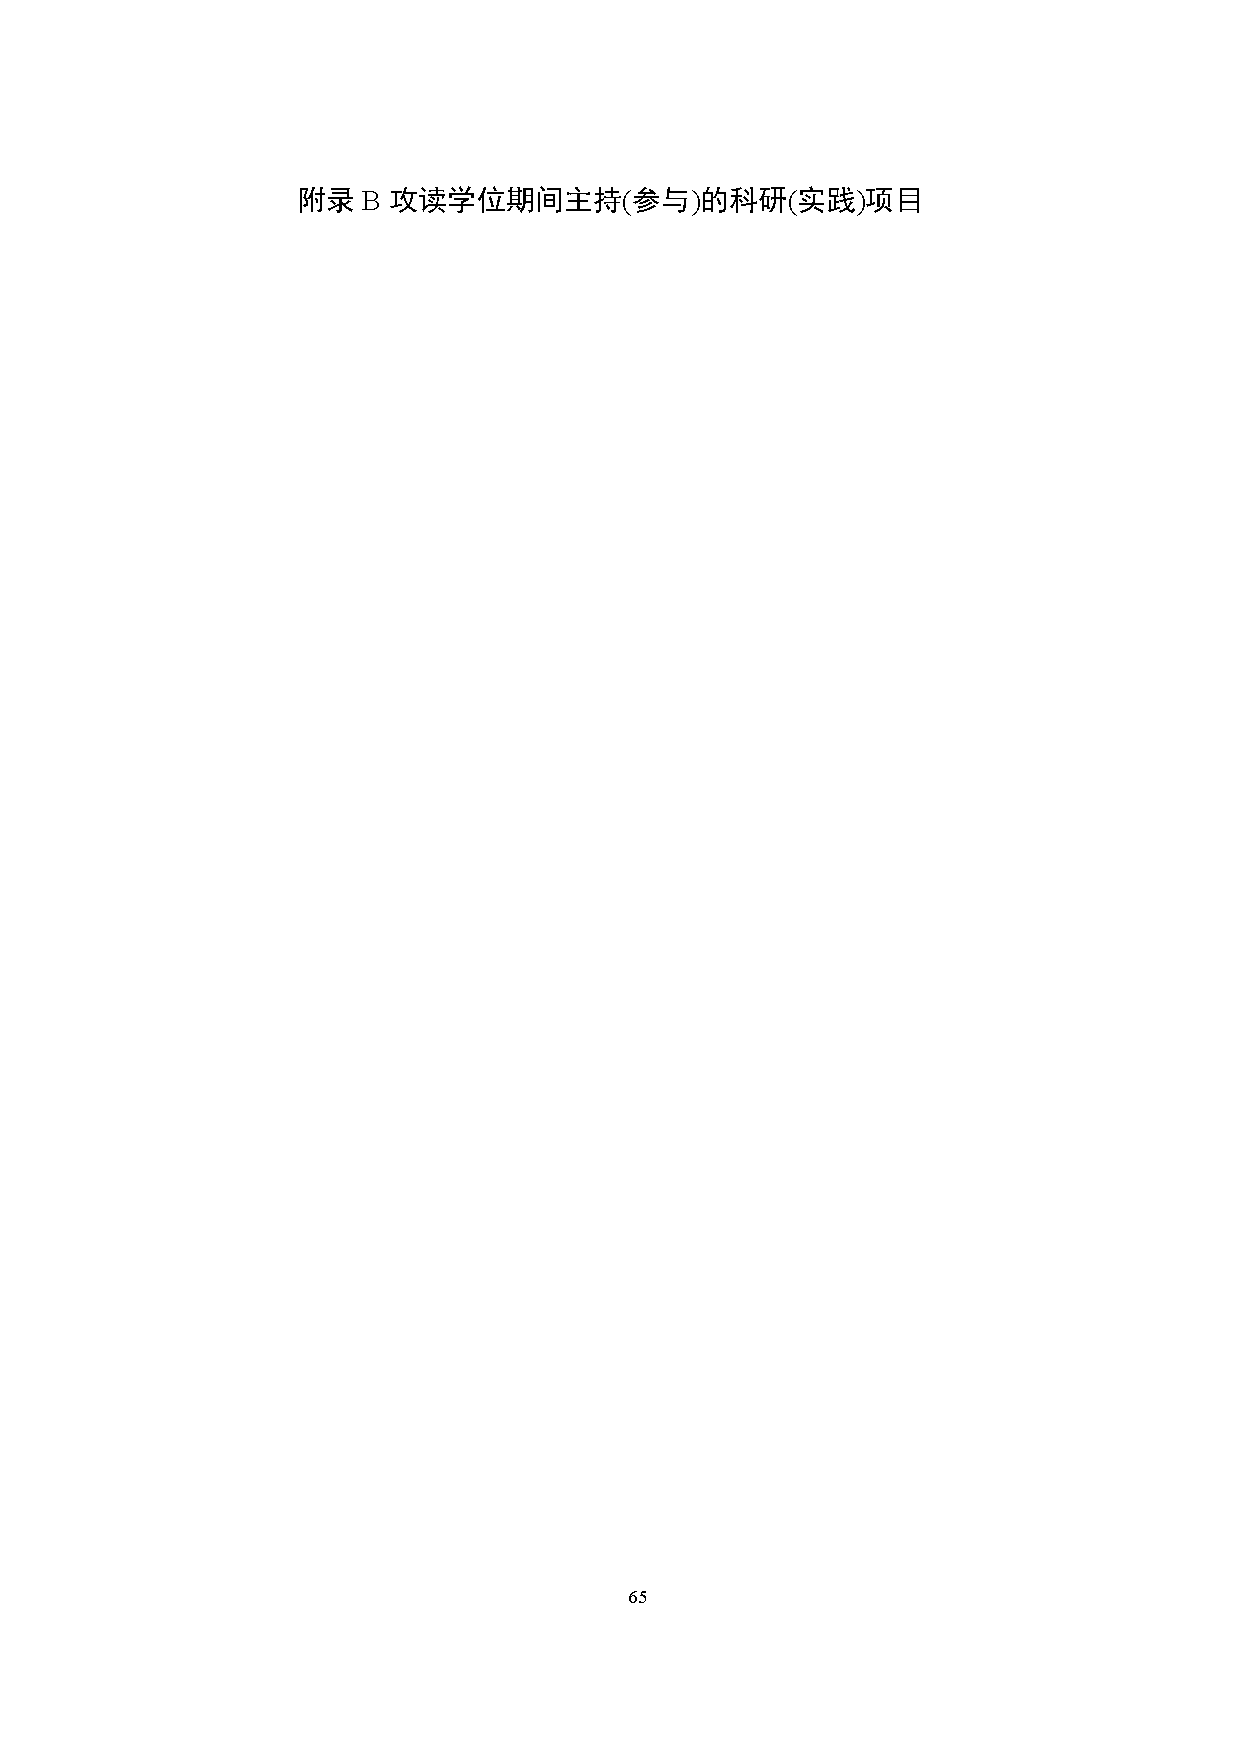
\includepdf[pages=-]{data/fub.pdf}

\end{document}
